%  This section should be divided by subheadings. Materials and
%  Methods should be described with sufficient details to allow others
%  to replicate and build on published results. Please note that
%  publication of your manuscript implies that you must make all
%  materials, data, and protocols associated with the publication
%  available to readers. Please disclose at the submission stage any
%  restrictions on the availability of materials or information. New
%  methods and protocols should be described in detail while
%  wellestablished methods can be briefly described and appropriately
%  cited. Give the name and version of any software used.

% ◦ Research manuscripts reporting large datasets that are deposited
% ◦ in a publicly available database should specify where the data
% ◦ have been deposited and provide the relevant accession numbers. If
% ◦ the accession numbers have not yet been obtained at the time of
% ◦ submission, please state that they will be provided during
% ◦ review. They must be provided prior to publication.

\section{Experimental Section}

\subsection{Case Study: Autonomous Ground Support Equipment (AGSE) Robot}

This section briefly describes an Autonomous Ground Support Equipment
(AGSE) robot that we designed, built, and deployed for the 2014-2015
NASA Student Launch Competition \cite{NASA_SL}. Special emphasis is
given to the value of a rapid system prototyping methodology in the
design process and how it allowed the AGSE to overcome many of the
challenges and problems encountered during the competition.  We use
this example to demonstrate the utility of our integrated model-driven
component-based software tool suite.

%States the design requirements for the project
\subsection{Competition Requirements}

The NASA Student Launch Initiative \cite{NASA_SL} is a research-based
competition partnered with NASA's Centennial Challenges, and aims to
stimulate rapid, low-cost development of rocket propulsion and space
exploration systems.  Both collegiate and non-academic teams
participate in the 8-month competition cycle composed of design,
fabrication, and testing of flight vehicles, payloads, and ground
support equipment.

The purpose of the 2014-2015 competition was to simulate a Mars Ascent
Vehicle (MAV) and to perform a sample recovery from the Martian
surface. The requirements for this simulation were twofold: (1) Design
and deploy a system termed the Autonomous Ground Support Equipment
(AGSE) that independently retrieves a sample off the ground and stores
it in the payload bay of a rocket, and (2) launch the rocket to an
altitude of 3000 ft. before safely recovering the sample.


\subsection{AGSE Project Architecture}
%States how we meet those design requirements (related to the agse)
%components: robotic arm and payload bay "in order to accomplish X we used Y"
%robot behavior, workspace, and control
%payload bay behavior and design "controlled through serial port by agse, otherwise not part of the rosmod-based design process"
%state chart

The sample retrieval was accomplished using a robotic arm with
computer vision to find the sample and identify its orientation. After
successfully acquiring the sample, the system will then search for the
payload bay, identify its orientation, and place the sample within it.
The robot arm itself is a simple crane-style device akin to a
pick-and-place robot with a four-pronged gripper as the end effector.
It was designed to have a cylindrical workspace in order to most
efficiently access the ground around the system and rocket. It starts
in a known position and incrementally scans its workspace using a
built in camera. Image processing is performed to identify key
environmental features such as the sample and payload bay.  The
control flow in the AGSE software is shown in Figure
\ref{fig:AGSE-FlowChart}.

\begin{figure}[h]
	\centering
        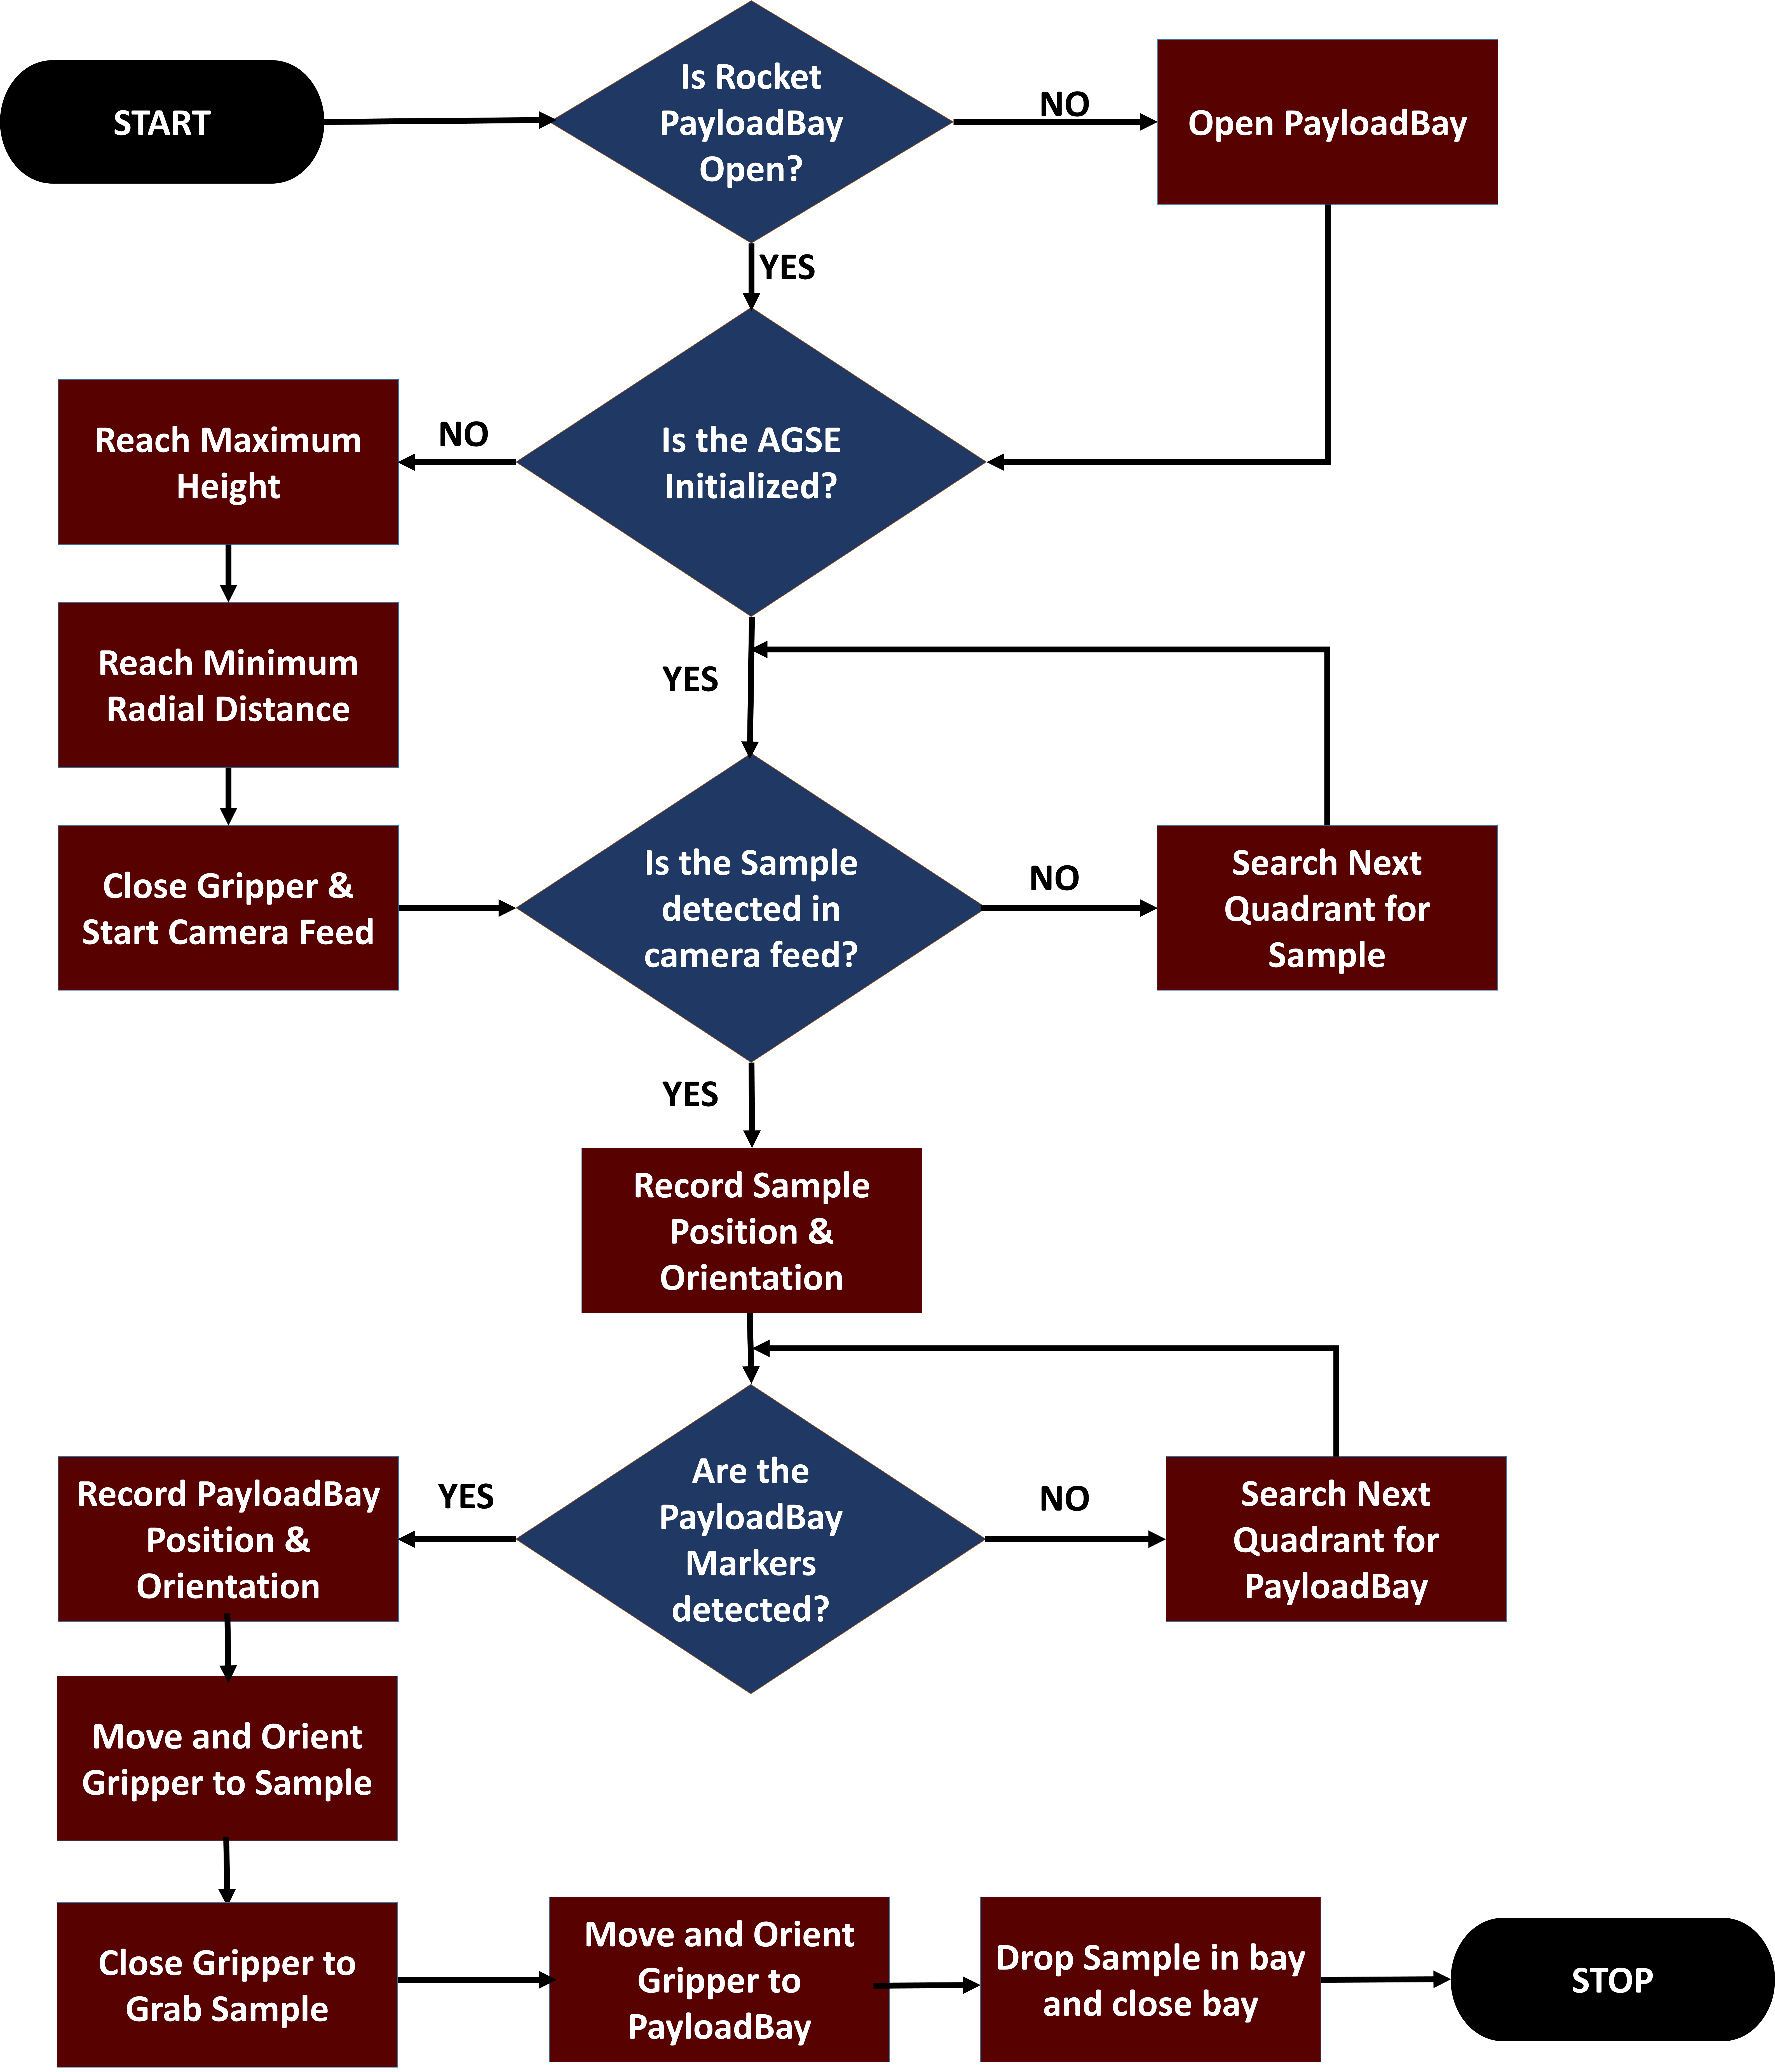
\includegraphics[width=0.8\textwidth]{Figures/AGSE-FlowChart.png}
	\caption{AGSE Control Flow Chart}
	\label{fig:AGSE-FlowChart}
\end{figure}

While the driving requirements of the competition were fixed, many of
the minor rules regarding AGSE performance, behavior, and safety
requirements evolved and were augmented throughout the course of the
competition. The volatile nature of these rules combined with the
short eight month duration of the build cycle precipitated the need
for rapidly adjustable design and fabrication processes. As such, an
iterative, modular, design-build-test approach was implemented in
order to concurrently develop as many components of the hardware and
software systems as possible. An initial AGSE prototype was
conceptualized from off-the-shelf components and the mechanical and
software systems were built in parallel, integrated, and tested. These
preliminary results were then used in future development to produce a
more ideal structure with greater positional accuracy and system
robustness.  Due to the modular nature of the system's design, it was
not necessary to immediately build a completely new second system, so
incremental improvements could be made on a specific subsystem (such
as the robot's gripper, any single degree of freedom, image
processing, motor control, etc.) as the design evolved.

\subsubsection{Distributed Deployment}

The AGSE robot is controlled by a distributed set of embedded
controllers. Figure \ref{fig:AGSE_Deployment} shows the high-level
design for the deployment architecture. There are three embedded
devices, each with its own responsibilities.  The reasons for the use
of multiple embedded controllers cooperating was two-fold: 1) given
the design decision to fully automate the robot to search the
workspace for both the sample and the payload bay, we needed an
embedded processor capable of performing image-based object detection
and 2) given the design of the robot to search a workspace with the
given degrees of freedom, we needed an embedded processor with the
required available General Purpose Input/Output (GPIO) and Special
Function Input/Output (SFIO) pins. 

To meet the first requirement, we selected the NVIDIA Jetson TK1, which is an embedded ARM controller
with 4+1 ARM cores and 192 CUDA cores, that consumes 10 W or less.
We could not use the Jetson to meet the second requirement since it
does not support enough GPIO to control the linear actuators and
retrieve feedback from them.  Furthermore, it lacks SFIO for encoder
pulse decoding.  Therefore, a BeagleBone Black was selected for the
motor control interface board because it has specific hardware for
decoding quadrature encoded pulses (QEP) and enough available GPIO for
controlling the linear actuators and reading limit switches.

Since one of the secondary requirements of the competition governed
pause control and state feedback to the operator of the AGSE (during
the competition execution), a second BeagleBone Black was introduced
which served to provide mechanical safety switches for pausing the
AGSE, LED panels indicating the state of the AGSE, and a touchscreen
showing what the AGSE sees as it searches the workspace for the sample
and the payload bay.  This BeagleBone Black resides the User Interface
Panel (UIP).

\begin{figure}[h]
	\centering
        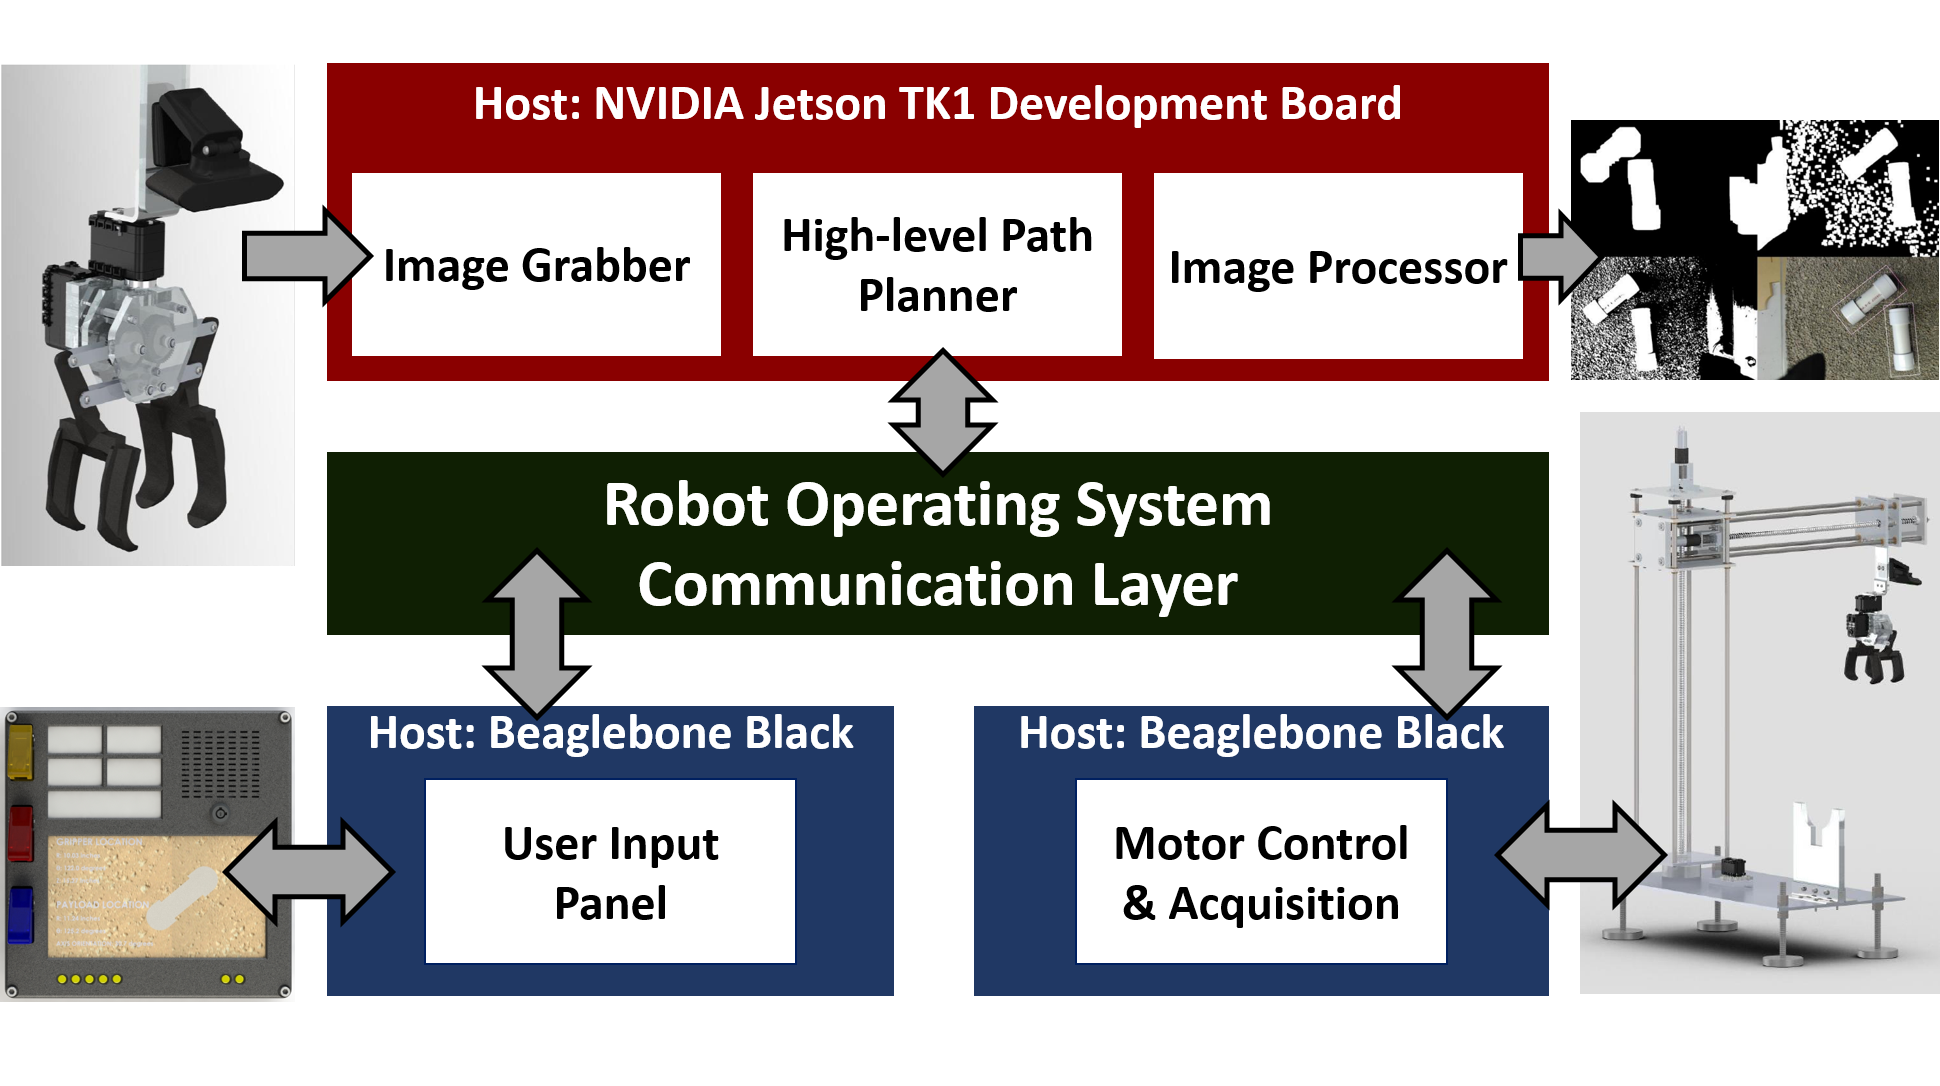
\includegraphics[width=\textwidth]{Figures/AGSE_Deployment.png}
	\caption{AGSE Package Deployment}
	\label{fig:AGSE_Deployment}
\end{figure}

The NVIDIA Jetson TK1 periodically fetches the latest webcam feed,
performs image processing and high-level path planning, and updates a
global state machine. The Beaglebone Black (BBB) mounted on top of the
robot performs power management, low-level motor control and feedback
processing. Lastly, the User Input Panel (UIP) houses a second
Beaglebone Black which reacts to user input through switches and
provides feedback through touchscreen display and LED panel
display. The UIP also responsible for keeping the user
informed about the real-time state of the AGSE and the current webcam
feed. Each of these controllers host multiple ROS nodes with ROSMOD
component executor threads periodically performing algorithmic
computations, calculating new robotic paths and communicating to
coordinate and maintain the AGSE state.

\subsubsection{Software Prototyping with ROSMOD}

\begin{figure}[h]
	\centering
        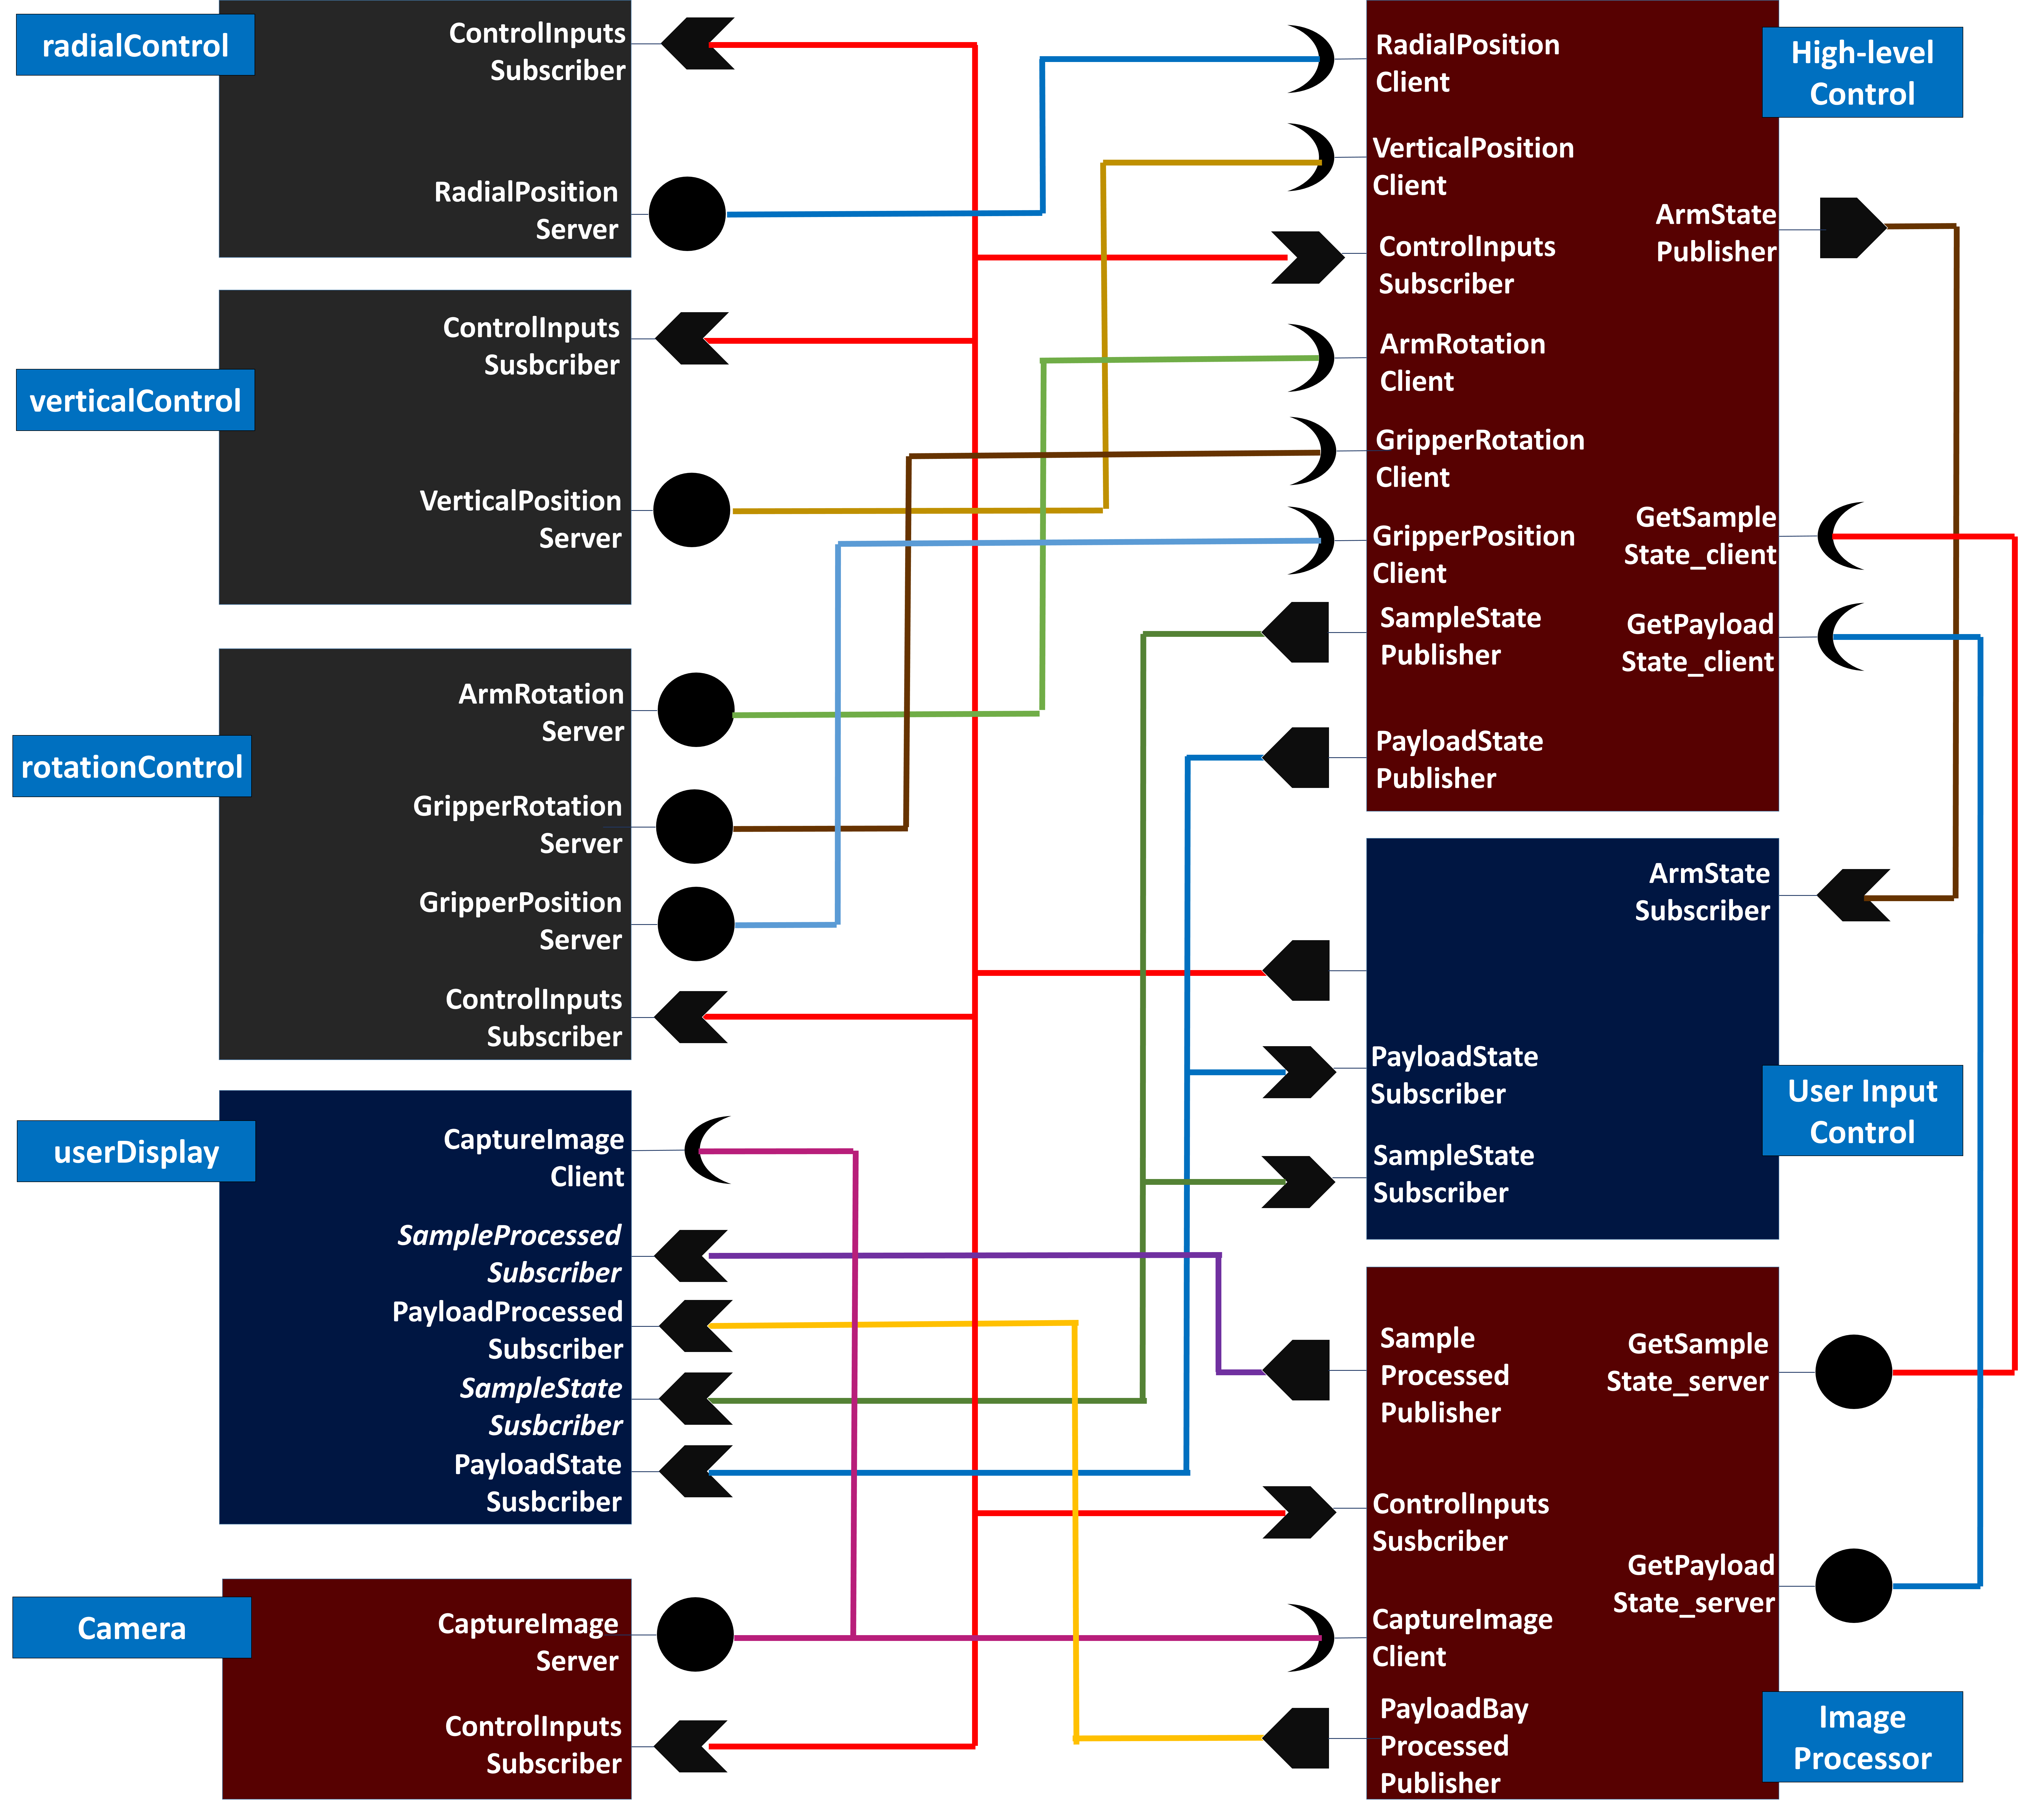
\includegraphics[width=\textwidth]{Figures/AGSE-Deployment.png}
	\caption{AGSE Component Assembly}
	\label{fig:AGSE}
\end{figure}

The AGSE software was iteratively designed and rapid prototyped using
our ROSMOD tool suite. The Software Model consists of 8 components
spread across three ROS packages - motor control, high-level state
machine control and image processing. Each package is characterized by
its local set of messages, service and interacting components. Note
that just as in ROS, packages can share messages so that components
can subscribe/publish/provide/require messages/services from other
packages. Figure \ref{fig:AGSE} shows the component assembly and
wiring as per the design. The \emph{radialControl} and
\emph{verticalControl} components are responsible for radial and
vertical actuation of the AGSE respectively. The
\emph{rotationControl} component is capable of controlling three servo
motors: (1) the base rotation servo, (2) the gripper rotation servo,
and finally the (3) gripper position servo that opens and closes the
robot gripper. A \emph{Camera} component deployed on the NVIDIA Jetson
TK1 provides a direct interface to the camera. Using the
\emph{CaptureImage\_Server}, the \emph{ImageProcessor} component
receives a snapshot of the camera feed for periodic processing
needs. This feed is also used by the \emph{userDisplay} component to
display the feed on the user input panel, as shown in Figure
\ref{fig:AGSE_Deployment}. The user input panel is the primary
interface between the ROSMOD applications and the user. The
\emph{userDisplay} component provides information to the user and the
\emph{userInputControl} receives data from the user, specifically to
read the various control switches on the panel e.g. the pause, alarm,
and debug switches. Lastly, a \emph{HighLevelControl} component
orchestrates the high-level state transitions and controls the
operation of the robotic arm. These transitions include commands such
as \emph{find\_payload\_bay}, \emph{find\_sample},
\emph{move\_to\_target} etc., each of which publishes messages to
other components to propagate the motor control commands.

The ROSMOD code generators enabled generation of nearly 60\% (6,000+
lines) of the total built code. As mentioned before, much of this code
includes port initialization, build system files, callback skeletons,
etc. that usually take up a significant amount of development time. As
developers, we had to fill in the missing pieces - the business logic
of the callbacks, completing the component interaction loops. This
code includes architecture-specific control, e.g. GPIO and encoder
readings, LED and switch settings, camera image acquisition, and
high-level control.

The final AGSE used in the 2014-2015 NASA SLI competition is shown in
Figure~\ref{fig:competition_AGSE}.

\begin{figure}[h]
	\centering
        \includegraphics[width=\textwidth]{./Figures/AGSE_Render.png}
	\caption{AGSE and rocket used in the 2014-2015 NASA SLI
          competition.  The UIP is shown in the bottom left of the
          picture, the Motor Control Board is on the top of the arm of
          the AGSE, and the NVIDIA Jetson is under the rocket.}
	\label{fig:competition_AGSE}
\end{figure}

